\documentclass[12pt,letterpaper, oneside]{book}
\usepackage[left=2.54cm, right=2.54cm, top=2.54cm, bottom=2.54cm]{geometry}


\usepackage[utf8]{inputenc}
\usepackage[T1]{fontenc}
\usepackage[spanish]{babel}

\usepackage{amsmath}
\usepackage{amsfonts}
\usepackage{amssymb}
\usepackage{makecell}
\usepackage{longtable}
\usepackage{physics}
\usepackage{units}

\usepackage{graphicx}
\usepackage{appendix}
\renewcommand{\appendixname}{Anexos}
\renewcommand{\appendixtocname}{Anexos}
\renewcommand{\appendixpagename}{Anexos}

\usepackage{fancyhdr}
\fancypagestyle{plain}{
	\lhead{}
	\fancyhead[R]{}
	\fancyhead[L]{}
	\renewcommand{\headrulewidth}{0pt}
	\fancyfoot{}
}

\pagestyle{fancy}
\fancyhead[R]{\thepage}
\fancyhead[L]{}
\renewcommand{\headrulewidth}{0pt}
\fancyfoot{}

\usepackage{tikz}
\usetikzlibrary{calc}

\author{J. Moisés Arias}
\title{Obtención de un modelo de supervivencia celular ante radiación ionizante desde primeros principios físicos}
\decimalpoint

\begin{document}
	\begin{titlepage}
		
		\begin{tikzpicture}[remember picture, overlay]
		\draw[line width = 4pt] ($(current page.north west) + (0.5in,-0.5in)$) rectangle ($(current page.south east) + (-0.5in,0.5in)$);
		\end{tikzpicture}
		
		\begin{center}
			%\vspace*{1cm}
			
			\Large \sc{\textbf{Universidad Nacional Autónoma de Honduras}}
			
			\vspace{0.5cm}
			\large{Tegucigalpa, Francisco Morazán, Honduras}\\
			\small{Septiembre - Diciembre 2023}
			
			\vspace{0.75cm}
			
			\begin{figure}[h]
				\centering
				\begin{tabular}{ccc}
				
\includegraphics[scale=1.56]{logotipos/logo3.jpg} & 
\includegraphics[scale=0.5]{logotipos/logo1.png} & 
\includegraphics[scale=0.44]{logotipos/logo4.png}
				\end{tabular}
			\end{figure}
			
			\vspace{0.75cm}
			\Large Tesis para acreditar el grado de licenciado en Física con énfasis en Radiaciones\\
			
			\vspace{1.25cm}		
			
			\large{J. Moisés Arias}\\
			\small{Escuela de Física, Facultad de Ciencias}
			
			\vfill
			
			\large{\textbf{Construcción de un modelo teórico de supervivencia celular ante radiación ionizante}}
			\vspace{0.75cm}
			
			\large Supervisor: M.Sc. Ángel Velásquez\\
			Departamento: Gravitación, Radiación y Altas Energías
		\end{center}
	\end{titlepage}
	
	\tableofcontents
	
	\chapter*{Introducción}
	\addcontentsline{toc}{chapter}{Introducción}
	
	Los modelos de supervivencia celular han sido objeto de estudio casi desde el inicio mismo de la radiobiología como una rama de estudio. El impacto de las radiaciones, en particular de las radiaciones ionizantes, en la salud del ser humano como de cualquier otro ser vivo constituyen al día de hoy un tema de arduo debate y gran interés científico. El tema no solo se remite al ámbito médico, donde está de más recalcar su relevancia, sino que afecta también a los ámbitos cotidianos desde el uso de la tecnología del hogar hasta los cuidados de la piel de implacables fenómenos de la naturaleza. 
	
	Los modelos de supervivencia celular buscan cuantificar una proporción de células o colonias de células que superan una cierta dosis de energía absorbida durante una interacción con una sustancia radiactiva o una fuente de energía espontánea, en su defecto. Estos modelos se presentan gráficamente como una curva que traza el decaimiento de una fracción de la población celular a medida que la dosis de energía aumenta durante un intervalo de tiempo. 
	
	Para fines clínicos, una curva de supervivencia celular dicta la calidad de un tratamiento terapeútico en pos de la tasa a la que se destruye el tejido canceroso mediante la acción de la radiación. Para fines de radioprotección las curvas de supervivencia celular nos pueden dar una pista de cuán riesgoso es permanecer en un espacio donde existe una amenaza radiológica. 
	
	Estas ecuaciones, o mejor dicho funciones, se han construido desde datos experimentales y los intentos por obtener un modelo de manera teórica, ya sea de forma heurística o desde primerios principios son virtualmente escasos en la literatura científica. Este trabajo aspira a dar un primer paso hacia la obtención de un modelo teórico o a lo sumo, semi-empírico. 
	
	Para formular la tasa de supervivencia celular en función de la dosis se recurrirá al marco de las interacciones de la radiación con la materia. En este conjunto de teorías se establecen las medidas de energía que pueden entregar las partículas neutras y cargadas a un medio durante su recorrido.
	
	Asociadas a estos mecanismos de interacción hay coeficientes que dictan la tasa a la cual la energía de las partículas es depositada en el medio. Estos términos formarán un rol importante en el modelo. 
	
	\chapter*{Objetivos}
	\addcontentsline{toc}{chapter}{Objetivos}
	
	\section*{Objetivo general}
	\begin{itemize}
		\item Determinar un modelo teórico desde primeros principios Físicos y Matemáticos sobre la supervivencia celular en tejidos enfermos y sanos ante la interacción con una fuente radiactiva en tratamientos terapéuticos contra el cáncer en general.
	\end{itemize}
	\section*{Objetivos específicos}
	\begin{itemize}
		\item Emplear métodos matemáticos propios de la Física en la obtención de un modelo teórico de supervivencia celular en radioterapias. 
		\item Implementar principios termodinámicos, electrodinámicos, nucleares y mecánico-cuánticos para la descripción cuantitativa de la respuesta celular y tisular a la radiación. 
		\item Simular computacionalmente las respuestas de un tejido a la radiación mediante la evaluación funcional del modelo. 
		\item Comparar los resultados teóricos con los registros experimentales disponibles en la literatura biomédica. 
	\end{itemize}
	
	\chapter{Fundamentos físico-biomédicos y alcances de la radiobiología}\label{fundamentos_fisico_biomedicos}
		\section{Cronología de la radiobiología}
		La Física y la Biología han crecido una de la mano de la otra desde el siglo pasado de forma acelerada. A esta conjunción [de Física y Biología] le llamamos \textit{Radiobiología} y consiste en el estudio de la acción de las radiaciones ionizantes en los seres vivos\cite{Hall.2000}. 
		
		Las radiaciones han sido vistas como una amenaza a la vida debido a graves catástrofes que se han suscitado en el pasada a raíz de la ignorancia sobre su naturaleza\cite{Prasad.1995}. No obstante, con el paso del tiempo se ha descubierto una serie de invaluables beneficios a la calidad de vida que yacen en el uso prudente y mesurado de las radiaciones. Estos van desde tratamientos médicos, medidas de seguridad en la ocupación médica y el tratamiento de alimentos para su preservación\cite{Prasad.1995}. 
		
		Los registros muestran que los primeros intentos formales por documentar los efectos de la radiación en el tejido vivo desde 1896 al margen del descubrimiento de los rayos X y la radiactividad\cite{Hall.2000}. Este trabajo consistió en el reporte de quemaduras en la piel, irradiación ocular y pérdida de vello. 
		
		Podemos recorrer una breve cronología del desarrollo de la radiobiología contemplando algunos de los más grandes hitos en las Ciencias de las Radiaciones. \textit{Hall} ofrece una breve línea temporal de la que se muestran en la tabla \ref{cronologia_radiaciones} algunos eventos relevantes para la discusión en esta tesis
		
		\begin{longtable}{rl}
			\hline
			1896 & \makecell[l]{Documentados los primeros efectos de los rayos X en forma de quemaduras y\\ depilación.}\\\hline
			1903 & \makecell[l]{Bergonie y Tribondeau presentan una \textit{ley} sobre radiosensibilidad con base en\\ actividad mitótica.\\ Se plantea por primera vez el uso de implantes de radio para tratar el cáncer.}\\ \hline
			1911 & \makecell[l]{Se reportan 5 trabajadores de las radiaciones afectados de leucemia.}\\\hline
			1915 & \makecell[l]{La \textit{Sociedad Británica Roentgen} hace propuestas para protección radiológica.}\\\hline
			1923 & \makecell[l]{Eugene Petry descubre el \textit{efecto oxígeno} con raíces de plantas.}\\\hline
			1927 & \makecell[l]{Se observan las primeras mutaciones por radiación en \textit{Drosophila.}}\\\hline
			1928 & \makecell[l]{Reportada la superioridad del tratamiento fraccionado para el cáncer humano.\\ Se Establece un Comité Internacional en Rayos X y Protección contra el Radio.}\\\hline
			1930 & \makecell[l]{Primera curva de supervivencia para bacterias expuestas a radiación.}\\\hline
			1933 & \makecell[l]{Se postula la importancia del oxígeno en la radioterapia por las observaciones\\ de sus efectos en la radiosensibilidad celular.}\\\hline
			1935 & \makecell[l]{Oficialmente se postula la importancia del oxígeno para la radioterapia.}\\\hline
			1940 & \makecell[l]{Propuesta del formalismo \textit{lineal-cuadrático} para la respuesta biológica\\ a la radiación.}\\\hline
			1952 & \makecell[l]{Se publica la primera medición del efecto oxígeno.}\\\hline
			1956 & \makecell[l]{Primera curva de supervivencia para radiación \textit{in vitro} en células de mamíferos.}\\\hline
			1959 & \makecell[l]{Primera curva de supervivencia \textit{in vivo} para células tumorales.}\\\hline
			1960 & \makecell[l]{Cambio de la forma de la curva de supervivencia debido a LET.}\\\hline
			1963 & \makecell[l]{Primera observación de variaciones en radiosensibilidad a través del\\ ciclo celular.\\ Primera demostración de que las células hipóxicas limitan la curabilidad\\ en tumores.}\\\hline
			1967 & \makecell[l]{Primera curva de supervivencia celular en cultivos de piel \textit{in vivo}}\\\hline
			1968 & \makecell[l]{Se da una clasificación de radiosensibilidad tisular.}\\\hline
			1971 & \makecell[l]{Primera curva de supervivencia celular para hipertermia.\\ Curva de supervivencia para médula ósea.\\Sensibilidad al calor a través del ciclo celular.}\\\hline
			1980 & \makecell[l]{Se publica la diferencia en la forma de curvas de supervivencia en tejidos\\ temprana y tardíamente responsivos.}\\\hline
			1981 & \makecell[l]{Se estiman los efectos hereditarios de la radiación en humanos.}\\\hline \caption{Breve cronología de algunos eventos singulares que marcaron hitos en el desarrollo de la radiobiología como punto de convergencia entre la Física y la Biomedicina. Los eventos son transcritos desde \cite{Hall.2000}.}	\label{cronologia_radiaciones}	
		\end{longtable}
		
		Hacia el año de 1897 ya se utilizaban los rayos X de Roentgen en medicina diagnóstica y en el tratamiento de anormalidades cutáneas, como la remoción de verrugas\cite{Hall.2000}. 
		
		El primer experimento radiobiológico registrado se debe a Becquerel cuando dejó descuidadamente un contenedor de radio en sus bolsillos; éste dejó un eritema en la zona de contacto que tardó varias semanas en sanar\cite{Hall.2000}. 
		
		Los efectos de la radiación fueron estudiados de inmediato por los Curie, quienes deliberadamente se provocaron quemaduras en sus brazos para observar el impacto de las sustancias radiactivas en el tejido vivo\cite{Hall.2000, Prasad.1995}. 
		
		No solo los descubrimientos en Física han representando un avance significativo en la Radiobiología. El desarrollo de la Biología en cuanto al conocimiento del ciclo celular y las características en sus etapas, ha abierto las puertas a comprender los mecanismos de radiosensibilidad en la materia viva\cite{Prasad.1995}. Los logros en el cultivo de tejido vivo \textit{in vitro} y los experimentos \textit{in vivo}, así como los estudios genéticos y celulares y bioquímicos han nutrido en gran medida las teorías radiobiológicas\cite{Prasad.1995}. 
		
		\section{Modelos de supervivencia celular}
		Sabemos que las células menos especializadas son más propensas a los efectos de la radiación, así mismo, los tejidos en crecimiento son más sensibles a dichos efectos\cite{Prasad.1995}.
				
		La \textit{radioterapia} juega un rol muy importante en el cuidado del cáncer y constituye en sí misma una disciplina de rápida evolución\cite{Mayles.2007}. Es en el contexto de la radioterapia que surge el interés por conocer el comportamiento de las células al absorber la energía transportada en las radiaciones\cite{Mayles.2007}. 
		
		En general el proceso mediante el cual las células captan la energía radiativa es más bien aleatorio, pues la deposición de la radiación se suscita a lo largo de trayectorias o recorridos sujetos a una medida de probabilidad por la inherencia cuántica de las interacciones de la radiación con la materia\cite{Mayles.2007}. 
		
		Para entender las tasas de supervivencia celular durante una terapia radiológica, es preciso comprender los mecanismos físicos y biológicos implicados en la deposición/absorción de energía por los tejidos. Este problema es, en fundamento, uno de interacciones de la radiación con la materia donde la termodinámica, mecánica cuántica y electrodinámica desempeñan un papel central. 
			
		Se define como muerte celular para células diferenciadas no-proliferantes al evento en el que la célula pierde su funcionalidad\cite{Hall.2000, Tubiana.1990}; para células proliferantes, la muerte celular ocurre cuando la célula pierde su integridad reproductiva\cite{Hall.2000, Tubiana.1990}. 
		
		A la luz de estas dos definiciones, se contempla que una célula cualquiera \textit{muere}, o experimenta citólisis, cuando pierde la capacidad de tener una descendencia indefinida\cite{Hall.2000, Tubiana.1990}. La \textit{teoría de objetivos} muestra que una célula precisa experimentar un mínimo número de golpes o eventos dañinos en el tratamiento antes de perder su integridad reproductiva\cite{Bleehen.2007}. 
		
		Los mecanismos de muerte celular pueden ser diversos. La \textit{apoptosis} es una forma de \textit{muerte programada}; mientras que la \textit{muerte mitótica} sucede cuando la célula pretende dividirse, mas no lo logra \cite{Hall.2000, Tubiana.1990}. 
		
			\subsection{Curva de supervivencia celular} 		
			Una \textit{curva de supervivencia celular} [CSC] describe la relación entre la dosis de radiación y la razón de células que no mueren bajo tal dosis\cite{Hall.2000, Tubiana.1990}. Esta se puede modelar para células \textit{in vivo} e \textit{in vitro}. Empero, cabe señalar que no es fácil deducir el comportamiento \textit{in vivo} de las células a partir de su respuesta a la dosis observada \textit{in vitro}\cite{Tubiana.1990}. 
			
			\textit{In vivo}, se espera que bajo la dosis correcta el número de células clonogénicas se vea reducido significativamente; decimos que el tumor o tejido enfermo se encuentra [localmente] bajo control\cite{Tubiana.1990}. 
			
			La obtención de CSC para tejido \textit{in vivo} es más lenta y cara, además de depender de una serie de hipótesis sobre el sistema; pues las observaciones son indirectas (registros de reacciones histológicas o respuestas tumorales)\cite{Tubiana.1990}.
			
				\subsubsection{La forma de una CSC}
				En general, una CSC puede mostrar uno de tres perfiles: exponencial con hombro, exponencial sin hombro o continuamente descendente con la dosis\cite{Bleehen.2007}. 
				
				La aparición de un hombro en la CSC sugiere un proceso de acumulación de daño durante el tratamiento radiativo\cite{Bleehen.2007}. La explicación de este hombro nace en la \textit{teoría de la reparación}. Durante el proceso de irradiación, las células pueden recibir daños subletales (estos son aquellos eventos surgidos por debajo del mínimo de golpes requerido para la muerte celular) y son capaces de recuperarse de tal daño\cite{Bleehen.2007}. A veces, el proceso de recuperación celular se satura a medida que las lesiones aumentan con la dosis; en este sentido, la pendiente de la CSC refleja la inducción de daños irreparables antes de que se sature la recuperación celular y la inducción de lesiones en la ausencia de reparación, después\cite{Bleehen.2007}. 
				
				La radioterapia fraccionada ensayada \textit{in vitro} muestra que la capacidad de reparación se debilita con el número de fracciones aunque los ensayos de supervivencia \textit{in vivo} muestran lo contrario\cite{Bleehen.2007}. Esto supone que el medio inmediato al tumor cumple una función dentro de su proceso de reparación, es deseado poder introducir esos efectos como parte de un modelo matemático de supervivencia celular.
				
				Describir cualitativamente una CSC suele ser tarea simple, pero dar una explicación biológica de las observaciones representadas en ella en términos biofísicos es otra historia\cite{Hall.2000}. Muchos modelos biofísicos han sido propuestos, así como teorías al lado de ellos, para explicar la forma de la CSC en mamíferos y casi todos logran ajustarse a los datos experimentales, pero nunca es posible elegir uno solo para representar el fenómeno en cuestión\cite{Hall.2000}.
				
				Algunas pautas simples para leer una CSC\cite{Hall.2000} son:
				\begin{enumerate}
					\item El eje horizontal es típicamente reservado para la dosis.
					\item El eje vertical es típicamente reservado para la $sf$ en una escala logarítmica.
					\item Las radiaciones con baja LET, muestran un comportamiento exponencial, inicialmente, hasta doblarse con el incremento de la dosis antes de mostrar una curva exponencial otra vez. 
					\item Las radiaciones con alta LET, muestran un comportamiento exponencial en todo su rango casi desde el inicio.
				\end{enumerate}

			\subsection{Métodos de medición de la tasa de células supervivientes}
				\subsubsection{CSC \textit{in vitro}.}
				Una prueba de viabilidad \textit{in vitro} es posible a varios grados de dificultad para la mayoría de células clonogénicas animales y humanas\cite{Tubiana.1990}. 
				
				Una CSC se construye a partir de la pérdida de la capacidad de replicación celular como una función de la radiación absorbida por el tejido vivo o dosis\cite{Hall.2000}. 
				
				Las técnicas modernas permiten realizar cultivos celulares \textit{in vitro} a partir de tumores o cualquier tejido celular regenerativo  mediante una suspensión con la encima tripsina\cite{Hall.2000}. Se conoce como tripsinización al proceso mediante el cual se disuelve la membrana celular por acción de la tripsina\cite{Tubiana.1990, Hall.2000}. 
			
				El método descrito por \textit{Tubiana et al} consiste en cultivar en condiciones bien definidas una muestra de células extraídas de una zona enferma y contabilizar las colonias a las que da lugar en su confinamiento. Como una medida para sostener la proliferación, cada ciertos días se retiran algunas colonias de la superficie del recipiente, se diluyen y re-implantan en otro frasco. Estas se llaman \textit{líneas celulares estables} y juegan un rol fundamental en radiobiología\cite{Hall.2000}.
			
				La población de células ahora puede ser irradiada en fase exponencial o en fase estacionaria, exclusive. En el primer caso, las células proliferan exponencialmente en el medio de cultivo; mientras que en el segundo caso las células se multiplican hasta ya no poder y entran en una fase de reposo\cite{Tubiana.1990}. 
			
				Después de la irradiación, las colonias presentan una reducción. Y es posible contabilizar el número de colonias presentes en el frasco, su razón con respecto a las colonias originales dan la fracción de supervivencia, $S$\cite{Tubiana.1990, Hall.2000}. 
			
				El experimento se realiza sobre un número conveniente de cultivos, de manera que pueda trazarse una CSC como una nube de dispersión\cite{Tubiana.1990, Hall.2000}. En el laboratorio se debe ajustar el número de células implantadas de manera que resulte un conjunto contable de colonias; muy pocas no serían estadísticamente significativas y demasiadas devolverían incertidumbres importantes por la agrupación de las colonias\cite{Hall.2000}.
				
				La \textit{eficiencia de las placas}, $pe$, es una medida que permite determinar el porcentaje de células sembradas que se convierten en colonias, de acuerdo con \cite{Hall.2000} este parámetro está sujeto a errores sistemáticos de tipo ambiental e instrumental y está dado por la siguiente expresión
				
				\begin{equation}
					pe=\frac{\textrm{Número de colonias formadas}}{\textrm{Número de células sembradas}}\times 100
				\end{equation}
				
				Se utiliza este factor para estimar cuántas células darán lugar a colonias durante el cultivo\cite{Hall.2000}, este número es más significativo en el cómputo de las tasas de supervivencia que el número de células implantadas.
				
				\textit{Hall} presenta una fórmula general para la fracción de supervivencia, $sf$, como:

				\begin{equation}
				sf=\frac{\textrm{Número de colonias formadas post-tratamiento}}{\textrm{Número de células sembradas $\times (pe/100)$}}
				\end{equation}
				
				Con todo este proceso de obtención de la CSC ignora el tipo de muerte celular, mitótica o programada\cite{Hall.2000}. Es una pregunta natural la cuestión de construir un modelo matemático que contemple la tasa de supervivencia celular en el contexto de la muerte durante mitosis o apoptosis. 
				
				\subsubsection{CSC \textit{in vivo}.}
				La supervivencia celular puede verse influenciada por las condiciones experimentales, las cuales difieren de un cultivo \textit{in vitro} a uno \textit{in vivo}\cite{Tubiana.1990}. \textit{In vivo}, el contacto entre células cumple con un rol regenerativo mucho más apreciable que en las células \textit{in vitro}\cite{Tubiana.1990}. 
				
				La supervivencia de las células malignas puede medirse a partir de su capacidad para inducir tumores o colonias metásticas\cite{Tubiana.1990}. Estudios \textit{in vivo} se han realizado con frecuencia en colonias intestinales y bazales\cite{Tubiana.1990}. 
				
				\paragraph{CSC en leucemia mediante disolución \newline}
				Históricamente, la primera CSC \textit{in vivo} fue concebida mediante la \textit{técnica de disolución} para un caso de leucemia linfocítica espontánea\cite{Tubiana.1990}. 
				
				El procedimiento descrito por \textit{Tubiana et al, 1990} consiste en preparar una suspensión de células individuales del tumor de origen e inyectarlas en diferentes grupos de animales. Se debe estimar el número de células sin irradiar que deben inyectarse para provocar un tumor en el 50\% de los ejemplares; este parámetro es denotado como TD50 y depende de la tasa de células clonogénicas en la suspensión y la efectividad del sistema inmune del receptor. Por último, la CSC [de las células malignas] se construye del aumento del TD50 a medida que la dosis aumenta previo a la extracción del tumor.   
				
				\paragraph{CSC en células hematopoyéticas totipotentes \newline}
				\textit{Tubiana et al, 1990,} comentan que esta técnica fue diseñada por Till y McCulloch tomando células de médula ósea de ratones e inyectarlas en especímenes previamente irradiados con $\unit[9]{Gy}$ de dosis. La intención de administrar tal dosis es provocar la muerte de casi todas las células hematopoyéticas de la zona irradiada sin inducir síndrome gastrointestinal en el paciente. Las células donadas entran al paciente por vía intravenosa y se acumulan en el bazo, donde ocuparán los sitios de las células antes irradiadas y formarán nódulos apreciables a simple vista. 
				
				Los nódulos son colonias o la progenie de las células totipotentes donadas y su tamaño es proporcional al número de células totipotentes inyectadas (medido en \textit{unidades formantes de colonias}, $CFU$). 
				
				La CSC [para las células totipotentes] se obtiene al irradiar al donante o a la suspensión de células por inyectar en una serie de dosis creciente. 
				
				\paragraph{CSC en criptas intestinales \newline}
				El procedimiento desarrollado por Withers y Elkind, consiste en irradiar totalmente o solo el abdomen de ratones con una dosis de $\unit[10]{Gy}$ a $\unit[15]{Gy}$ para matar una cantidad grande de células de las criptas intestinales. De 3 a 5 días después, los especímenes son sacrificados para contabilizar las criptas regeneradas en el yeyuno\cite{Tubiana.1990}. 
			
			\subsection{Los principales modelos de CSC}
			La supervivencia celular ante la radiación ionizante presenta formas gráficas distintas según el tipo de célula modelada\cite{Tubiana.1990}. Múltiples factores pueden influir en la dinámica de la dosis absorbida y sus efectos en el tejido tales como la fase del ciclo celular, la función de la célula y el reino biológico al que pertenece el ejemplar\cite{Tubiana.1990}.
			
			Las tasas de supervivencia que se muestran a continuación son empleadas bajo condiciones de referencia que involucran rayos X o gamma en dosis únicas cortas bajo condiciones bien oxigenadas. 
			
			\subsubsection{Curvas exponenciales de supervivencia}
			En mamíferos, las CSC muestran un comportamiento exponencial en el que es apreciable un hombro, por lo general se grafican en escalas logarítmicas o semiautomáticas para dejar ver el comportamiento lineal con la dosis\cite{Mayles.2007, Tubiana.1990}. 
			
			Un modelo exponencial típico es el de la forma
			
			\begin{eqnarray}
			S(D)=e^{-\alpha D}=e^{-D/D_0} \label{exponencial_csc_dosis_lineal}
			\end{eqnarray}
			
			Con $D_0=1/\alpha$ como una \textit{dosis letal media}, que representa la cantidad de energía por unidad de masa a la cual la $sf=e^{-1}=37\%$; también se le denota por $D_{37}$\cite{Tubiana.1990} tal como se hace con las dosis para lograr una supervivencia del 90\% y del 50\%, $D_{90}$ y $D_{50}$ respectivamente\cite{Mayles.2007}. La tasa de supervivencia en escala logarítmica prueba ser una función lineal de la dosis $D$:
			
			\begin{eqnarray}
				\log(S) = -\alpha D=-D/D_0 \label{logaritmica_csc_dosis_lineal}
			\end{eqnarray}
			
			En las células de mamíferos, la CSC puede presentar un hombro que con el aumento de la dosis desaparece para dar lugar a una curva lineal. La extrapolación de dicha línea hacia las ordenadas da lugar a un \textit{número de extrapolación} $n$\cite{Tubiana.1990}. El valor de dosis que corresponde en las abscisas a la intersección de la extrapolación con $S=1.00$ se le denota como $D_q$ y recibe el nombre de \textit{dosis cuasi-umbral}\cite{Tubiana.1990}.  
			
			\subsubsection{Curvas de supervivencia dadas por teoría objetivo}
			En el marco de la teoría objetivo, la supervivencia celular está sujeta a la eventualidad de un golpe letal. El número de tales golpes letales ve un aumento con la dosis, significando una probabilidad mayor de muerte celular tras $N$ eventos\cite{Tubiana.1990, Hall.2000}.
			
			Visto de esta forma la tasa de supervivencia está sujeta a la razón de eventos letales por número de células, $p$:
			
			\begin{eqnarray}
				S=e^{-p} \label{exponencial_csc_golpesletales}
			\end{eqnarray}
			
			Al igual las ecuaciones \ref{exponencial_csc_dosis_lineal} con \ref{exponencial_csc_golpesletales} se puede verificar que $1/D_0$ corresponde a un valor de $p/D$\cite{Tubiana.1990}.
			
			De acuerdo con \textit{Tubiana et al, 1990}, se debe entender que una célula contiene $n$ objetivos los cuales pueden ser desactivados por el tránsito de una partícula cargada; la desactivación de $n-1$ objetivos se corresponden con una serie de eventos subletales y el enésimo evento, el letal, desata la muerte celular. 
			
			Para un escenario muerte celular por un sólo golpe en múltiples objetivos, la tasa de supervivencia se calcula en función de la dosis sujeta a un parámetro de objetivos precisados para un evento letal:
			
			\begin{equation}
			S(D,n)=1-\left(1-e^{-D/D_0}\right)^n \label{csc_eventos_dosis}
			\end{equation}
			
			La función dada en \ref{csc_eventos_dosis} sugiere que la probabilidad de que un objetivo padezca daño es $1-e^{-D/D_0}$ y la probabilidad de dañar a $n$ objetivos en una célula, y por ende matarla, está dada por $(1-e^{-D/D_0})^n$\cite{Tubiana.1990}. Al número $D_0$ se le puede asimilar como la radiosensibilidad de $n$ objetivos subletales por célula\cite{Mayles.2007, Tubiana.1990}.  
			
			Por otra parte, un modelo exponencial cuadrático en la dosis es empleado para describir tasas de supervivencia en dinámicas de dos golpes en un objetivo singular\cite{Tubiana.1990}. El modelo es como sigue
			
			\begin{equation}
				S(D)=e^{-\beta D^2} \label{csc_dos_golpes}
			\end{equation}
			
			El parámetro $\beta$ está asociado a la probabilidad de producir un evento subletal\cite{Bleehen.2007, Tubiana.1990}. Los modelos en las ecuaciones \ref{csc_dos_golpes} y \ref{csc_eventos_dosis} funcionan bien para dosis relativamente altas, no así para dosis bajas ya que sus gráficas presentan una nula pendiente inicial sugiriendo cero mortalidad a pequeñas dosis\cite{Tubiana.1990}.  
			
			Un modelo a dos componentes surge de suponer los modos de muerte celular como eventos independientes, dando que la probabilidad de supervivencia $S(D)$ es el producto de \ref{logaritmica_csc_dosis_lineal} y \ref{csc_eventos_dosis}\cite{Tubiana.1990}, esto es
			
			$$S(D)=S_1S_n$$
			
			Donde 
			
			$$S_1=e^{-D/_1D_0}$$
			
			es la fracción de supervivencia para eventos letales de golpe singular y el coeficiente $_1D_0$ se relaciona a la probabilidad de una lesión letal directa. Y el factor
			
			$$S_n=1-(1-e^{-D/_nD_0})^n$$
			
			denota la fracción de supervivencia bajo la acumulación de eventos subletales con $_nD_0$ como coeficiente de producción de lesiones subletales. 
			
			La expresión resultante es:
			
			\begin{equation}
				S(D)=e^{-D/_1D_0}\left[1-(1-e^{-D/_nD_0})^n\right]\label{csc_onehitlethal_nsublethal}
			\end{equation}
			
			Una expresión alternativa, es el modelo lineal cuadrático
			
			\begin{equation}
				S(D)=e^{-(\alpha D + \beta D^2)}\label{csc_linear_quadratic_model}
			\end{equation}
			
			Los coeficientes $\alpha$ y $\beta$ de la ecuación \ref{csc_linear_quadratic_model} se relacionan, respectivamente, a los dos modos de muerte celular. 
			
			La razón $\alpha/\beta$ da un criterio para su importancia relativa en el proceso\cite{Tubiana.1990}. Un valor alto del índice $\alpha/\beta$ se asocia a una curva [casi] exponencial mientras que los valores bajos corresponden a un hombro ancho en la curva\cite{Tubiana.1990}, esto es, la ocurrencia de una acumulación de daño.
						
		\section{Efectos de las radiaciones en el tejido vivo}
		Cuando una célula conserva su integridad reproductiva a pesar de la dosis, puede producir una colonia (gran número de clones); a estas células se les llama \textit{clonogénicas}\cite{Hall.2000}.
		
		Una célula se considera viable o superviviente cuando, después de la irradiación, es capaz de generar un clon (o colonia) de 50 células o más\cite{Tubiana.1990}.
		
		Con base en la jerarquía celular encontramos a las células que conforman aquellos sistemas tisulares \textit{sanos} como restauradoras del cuerpo\cite{Mayles.2007}. Las células responsables de provocar carcinomas son precisamente derivadas de esa clase de tejidos; tales estructuras mantienen muchas de las propiedades de los tumores no-diferenciados\cite{Mayles.2007}. 
		
		La radiación se deposita en el tejido vivo mediante interacciones de las partículas constituyentes de las emisiones radiantes con los bloques estructurales de la materia [átomos y moléculas]\cite{Hall.2000, Tubiana.1990, Mayles.2007}.
		
		\subsection{Mecanismos de muerte celular} 
		Existe una cantidad abundante de evidencia, aunque circunstancial, por la cual sostener que la mayor sensibilidad a la radiación yace en el núcleo celular en vez del citoplasma\cite{Bleehen.2007, Hall.2000}. 
		
		El ADN contenido en los cromosomas es el objetivo principal para conseguir una letalidad radio-inducida, de acuerdo con múltiples estudios experimentales\cite{Hall.2000, Mayles.2007}. El daño se suscita mediante rupturas de las cadenas de ADN, las cuales pueden ser reparadas por una variedad de encimas\cite{Bleehen.2007}.			
		
		Los mecanismos de muerte celular conocidos son la apoptosis o muerte celular programa y la muerte mitótica. 
		
			\subsubsection{Apoptosis}
			La apoptosis es dependiente del tipo de célula; algunas presentan una mayor disposición a padecerla y en algunas otras no ocurre en lo absoluto\cite{Hall.2000}.
			
			Se ha reconocido que el proceso consiste en un aislamiento de la célula con respecto a sus vecinas acompañado por una fragmentación de su ADN cromosómico\cite{Hall.2000}. 
			
			A continuación, la célula se encoje y se divide en partes pequeñas portadores de citoplasma o fragmentos del núcleo o ambas limitadas por una membrana\cite{Hall.2000}.
			
			\subsubsection{Muerte mitótica}
			Esta es tan importante como la apoptosis y para ciertas células es el único canal por el cesan sus funciones\cite{Hall.2000}. La muerte mitótica es la razón principal por la cual el daño se manifiesta en diferentes momentos para diferentes tejidos\cite{Bleehen.2007}. 
			
			La célula muere cuando intenta dividirse, pero no lo logra debido a la fragmentación de su ADN\cite{Hall.2000, Bleehen.2007}. A bajas dosis, la célula puede dividirse hasta un par de veces antes de morir; son las altas dosis las que generan el daño más severo\cite{Bleehen.2007}. 
			
			Las aberraciones cromosómicas juegan un rol importante en este evento y su inducción por radiación tiene una medida de probabilidad dependiente de la dosis\cite{Hall.2000}. 
			
			Los efectos de la radiación a nivel del núcleo celular se ven reflejados en el modelo lineal-cuadrático. Ambos mecanismos tienen una contribución conjunta en la medición de la supervivencia en función de dosis, $S=S(D)$\cite{Hall.2000}.
			
		\subsection{Fases celulares y radiosensibilidad}
		Las células proliferan mediante la mitosis y el intervalo transcurrido entre divisiones sucesivas se llama tiempo del ciclo celular\cite{Hall.2000}. Durante ese período la célula pasa por 4 etapas cíclicas: mitosis, fase $\textrm{G}_1$, síntesis de ADN, $\textrm{G}_2$; donde las fases G conciernen a períodos de aparente inactividad entre los dos eventos mayores\cite{Hall.2000}.
		
		Las células en diferentes etapas del ciclo celular presentan distintas respuestas a la radiación\cite{Bleehen.2007, Tubiana.1990}. La fase mitótica se caracteriza por mostrar una gran radiosensibilidad, mientras que lo opuesto sucede en la fase de síntesis de ADN o fase S y en las fases $\textrm{G}_1$ y $\textrm{G}_2$ la radiosensibilidad es intermedia\cite{Bleehen.2007}. 
		
		La duración de cada fase del ciclo celular puede variar de un tipo de célula a otra\cite{Hall.2000, Bleehen.2007}. En células donde, por ejemplo, la fase $G_1$ es larga se puede apreciar una radiosensibilidad distinta en diferentes momentos de la fase\cite{Bleehen.2007}.	
		
		\subsection{El efecto del oxígeno}
			El depósito de energía en la materia viva por radiación se da en la producción de radicales libres altamente reactivos; estos reaccionan con oxígeno molecular para formar peróxidos capaces de fijar el daño en una forma letal\cite{Bleehen.2007}.
			
			Experimentos han mostrado que el \textit{efecto del oxígeno} es más duradero cuando el medio intracelular es privado de tioles\cite{Bleehen.2007}. En este sentido, se ha propuesta que modificar los niveles de tioles en el medio intracelular es una vía para aumentar la sensibilidad de las células a la radiación\cite{Bleehen.2007}. 
			
			La respuesta de un tejido a la radiación es altamente dependiente de la presencia de oxígeno\cite{Bleehen.2007, Mayles.2007}; las células hipóxicas pueden ser hasta 3 veces menos sensibles a la radiación que sus contrapartes oxigenadas\cite{Bleehen.2007}. 
			
			La forma de la CSC para una muestra de tejido mamífero puede variar dependiendo de la proporción de oxígeno presente en la muestra\cite{Bleehen.2007, Mayles.2007, Tubiana.1990}; los análisis experimentales detrás de la obtención de CSC mediante regresiones de $sf-versus-dosis$ muestran que la hipoxia puede ralentizar severamente el progreso de la tasa de supervivencia con el aumento de la dosis. Para ilustrarlo, \textit{Mayles et al, 2007} usa una gráfica comparativa de los efectos del oxígeno en $S(D)$ aquí presentada en la figura \ref{oxic_hypoxic_sc_Mayles2007}
			
			\begin{figure}[h!]
				\centering
				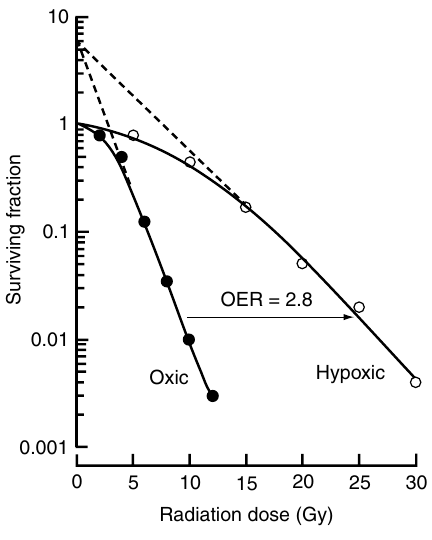
\includegraphics[scale=0.50]{imagenes/oxic_hypoxic_sc_Mayles2007.png}
				\caption{Curvas de supervivencia celular dadas como fracción de supervivencia en función de la dosis para células ricas en oxígeno y células pobres en oxígeno. Fuente: \textit{Handbook of Radiotherapy Physics - Mayles et al, 2007}.}\label{oxic_hypoxic_sc_Mayles2007}
			\end{figure}  
		
		La presencia de oxígeno en el medio puede mejorar los efectos de la radiación y esto se aprecia en la reducción de la dosis isoefectiva\cite{Mayles.2007}. Se define la \textit{tasa de mejoramiento por oxígeno}, OER por sus siglas en inglés, como la razón de dosis de radiación en hipoxia con respecto a la dosis en aire necesaria para alcanzar el mismo efecto biológico\cite{Mayles.2007, Smith.2000}. 
		
		El efecto del oxígeno, cuantificado por el OER, puede verse magnificado o reducido según el tipo de radiación y el ciclo celular, así como por el LET de la fuente\cite{Hall.2000}. 
		
		\subsection{Las 5 R de la radioterapia}
			Se ha probado experimentalmente que la aplicación fraccionada de la radiación tienen a mejorar el tratamiento\cite{Mayles.2007} y que la optimalidad del tratamiento está sujeto a la habilidad de las células para regenerar daños subletales (SLD) y potencialmente letales (PLD)\cite{Bleehen.2007}. 
			
			En la práctica radioterapeútica, se busca no solo reducir el área enferma, sino conseguir, en adición, un daño mínimo en el tejido sano vecino\cite{Mayles.2007}. 
			
			Los criterios de selectividad para implementar un tratamiento terapéutico con radiaciones toman en cuenta la distribución de la dosis y los efectos biológicos \textit{espaciales} tanto como \textit{temporales}, al igual que los tiempos de respuesta celular\cite{Mayles.2007}.
			
			\textit{Mayles et al, 2007} resume los factores que influencian la respuesta de un tejido neoplástico normal a la radioterapia fraccionada y son conocidos como \textit{las 5 R de la Radioterapia}:
			
			\begin{enumerate}
				\item \textbf{Reparación}: horas después de someterse a radiación ionizante, las células pueden pasar por un proceso de recuperación. 
				\item \textbf{Re-ordenamiento}: las células supervivientes progresarán hacia una fase resistiva del ciclo celular previo a desarrollar una fase más sensible a la radiación. 
				\item \textbf{Repoblación}: en el curso de 4 a 6 semanas posteriores a la radioterapia, aquellas células supervivientes pueden dar lugar a nuevas colonias. 
				\item \textbf{Re-oxigenación}: durante el tratamiento radioterapeútico las células hipóxicas podrán soporta la fracción de radiación. Al aumentar su influjo de oxígeno, se volverán más sensibles a la radiación. 
				\item \textbf{Radiosensibilidad}: no todas las células responden con el mismo grado de afinidad a la radiación, esto es, diferentes tejidos tienen una tendencia más fuerte a cesar sus funciones (operativas o reproductivas) ante la incidencia de radiación ionizante. 
			\end{enumerate}
		
		Idealmente, para construir un modelo teórico exitoso de la supervivencia celular como una función de la dosis, estos procesos biológicos deben incluirse de forma cuantitativa en el cálculo del número o fracción de colonias supervivientes. En ese sentido, se espera que los parámetros representativos de estos fenómenos aparezcan como factores o términos aditivos afectando la medida de dosis. 
		
		Cuantificar estos procesos ameritaría reconocer el efecto que tiene la radiación ionizante en las células objetivo en términos de la detención de sus funciones. Lo que requiere identificar la probabilidad de que una célula vea impedida su reproducción o trabajo en el tejido después de una interacción letal con la radiación. 	
	
	\chapter{Marco físico para la determinación de un modelo de supervivencia celular}
	Debido a que el problema de la supervivencia celular radica en la absorción de energía [ionizante], la construcción de un modelo matemático que considere la dosis como un causante de la reducción del tejido canceroso es, en principio, una cuestión termodinámica. 
	
	Los agentes portadores de la radiación ionizantes serían \textit{corpúsculos} u \textit{ondas electromagnéticas}. En el marco de las interacciones de la radiación con la materia, se estudian tanto la incidencia de partículas gobernadas por la mecánica cuántica como la transmisión y absorción de ondas electromagnéticas, continuas por naturaleza.
	
	El \textit{principio de complementariedad} de la mecánica cuántica sostiene que la radiación electromagnética es modelable desde una perspectiva corpuscular. Y así, el logro del objetivo general de este trabajo radica en determinar un modelo de supervivencia [celular] a partir de la energía deposita en la materia por interacciones con partículas elementales. 
	
	Observaciones desde la fisicoquímica y bioquímica necesitan ser tomadas en cuenta dentro de las condiciones o forma del modelo; pues estos aspectos gobiernan la naturaleza de la interacción de las radiaciones con la materia viva\cite{Bleehen.2007}. 
	
	Los parámetros de atenuación o absorción de la radiación ionizante dependerán de la identidad química de los objetivos además de la magnitud de la energía portada por el haz\cite{Mayles.2007,IAEA.2005,Podgorsak.2016}.
	
	De acuerdo con \cite{Mayles.2007} la deposición de energía por radiación en el tejido es, esencialmente, estocástica. Este proceso se desarrolla a través de colisiones a lo largo de un recorrido de longitud y direcciones aleatorias. Además, \cite{Mayles.2007} advierte que para valores pequeños de la masa del tejido, las fluctuaciones en la absorción se hacen más aparentes; de esta manera, existe una masa crítica a partir de la cual el comportamiento aleatorio del depósito de energía es más evidente a medida que la masa se reduce.
	
	Una manera de palear este problema es contemplando valores medios de energías y fluencias energéticas\cite{Mayles.2007, Podgorsak.2016}. De esta manera, los modelos matemáticos pretenden un acercamiento más bien determinista cuyas estimaciones se cotejan bastante bien con la experimentación\cite{Podgorsak.2016}.  
	
	\section{Interacciones de la radiación con la materia}
	La radiación corpuscular interactúa de maneras diferentes con la materia según se trate de partículas cargadas o neutras. Factores tales como el rango y la deposición de energía se ven afectados naturalmente. 
	
	Para empezar se construirá un modelo para rayos X y rayos $\gamma$, los cuales se contemplan como formas de radiación con baja LET\cite{Podgorsak.2016}. Se precisa formular el problema dentro de la clasificación de radiación ionizante, pues el objetivo es conseguir la tasa de supervivencia ante la absorción de energía suficiente para desdoblar cadenas de ADN, lo que implica impactos letales\cite{Mayles.2007, Tubiana.1990}. 
	
	El proceso de absorción de la energía electromagnética portada por los fotones depende tanto de la energía misma de los fotones como del número atómico del material absorbente o atenuador\cite{IAEA.2010, Mayles.2007}. Los efectos biológicos se suscitan debido a la absorción o dispersión de los rayos X o los rayos $\gamma$ en colisiones con los átomos de los tejidos\cite{IAEA.2010, Mayles.2007}. 
	
	Los siguientes procesos son los principales mecanismos de transferencia de energía de fotones a materia: absorción fotoeléctrica, dispersión Compton y producción de pares\cite{IAEA.2010,Podgorsak.2016}. 
	
	En el primer caso, así como el tercero, el fotón desaparece por completo al ceder su energía en la interacción, mientras que en el segundo casa se dispersa incoherentemente\cite{IAEA.2005}.
	
	Factores importantes de atenuación de la radiación electromagnética deben agregarse al modelo, estos son los coeficientes de transferencia energética, $\mu_{tr}$, y el coeficiente de absorción $\mu_{ab}$, definidos como
	
	\begin{eqnarray}
		\mu_{tr}&=\mu \frac{\bar{E}_{tr}}{h\nu}\\
		\mu_{ab}&=\mu \frac{\bar{E}_{ab}}{h\nu}
	\end{eqnarray}
	
	 \noindent El primer coeficiente, de acuerdo con \cite{Podgorsak.2016}, corresponde a una medida de la transferencia de energía a los electrones (y anti-electrones) en las interacciones fotón-átomo; puede evaluarse independiente de la densidad como un coeficiente de transferencia de energía másico $\mu_{tr}/\rho$. En cuanto al segundo, \cite{Podgorsak.2016} explica que hace referencia a una medida de energía absorbida en el medio y puede independizarse de la densidad como un coeficiente másico de la forma $\mu_{ab}/\rho$. 
	 
	 Los términos $\bar{E}_{tr, ab}$ son energía media transferida a las partículas cargadas del atenuador y la energía media depositada por las partículas cargadas en el atenuador\cite{Podgorsak.2016, IAEA.2005}. 
	
	 La energía transferida y la energía absorbida, en el sentido de \cite{Podgorsak.2016}, deben entenderse como la energía transferida a la energía cinética de las partículas cargadas con las que interactúan los fotones incidentes y la energía transferida al medio por las partículas cargadas secundarias producidas por la interacción, respectivamente. Por lo tanto, se refieren a dos procesos muy diferentes. 
	 
	 En el manual de \cite{IAEA.2005} se define $\mu$ como un factor de atenuación lineal dependiente de la energía del fotón y la especie química. En \cite{Mayles.2007}, el coeficiente de atenuación lineal dicta la probabilidad por unidad de longitud para una interacción y es una función de la sección eficaz atómica total:
	 
	 $$\mu=N \sigma_{tot}$$
	 
	 \noindent donde el parámetro $N$ dicta el número de entidades objetivos por unidad de volumen. Se define en función de la identidad del atenuador (su número másico, $A$ y densidad, $\rho$):
	 
	 $$N=\frac{N_A}{A}\rho$$	 
	 
	 La intensidad de un haz de fotones mono-energético está dado entonces por:
	 
	 \begin{equation}
	 	I(x)=I(0)\exp(-\mu(\nu, Z)x)\label{photon_beam_intensity}
	 \end{equation}
	 
	 De acuerdo con \cite{IAEA.2005}, un fotón tendrá diferente probabilidad de interactuar con una muestra material por un modo u otro según sea su energía y el número atómico de la muestra. 
	 
	 Para muestras orgánicas, las cuales interesan en este estudio, así como otra sustancia compuesta en general, los factores de atenuación son computados con el número atómico efectivo de la muestra\cite{IAEA.2005}. Se denota al número atómico efectivo con $Z_{eff}$ y para fotones de baja energía está definido por
	 
	 \begin{equation}
	 	Z_{eff}=\left[\sum_{i}a_i Z_i^{3.5}\right]^{1/3.5}\label{numero_atomico_efectivo}
	 \end{equation}
	 
	 \noindent y para fotones de mega-voltaje y haces electrónicos, se define por
	 
	 \begin{equation}
	 	Z_{eff}=\frac{\sum_{i}a_i \frac{Z_i^2}{A_i}}{\sum_{i}a_i \frac{Z_i}{A_i}}
	 \end{equation}
	 
	 \noindent donde $a_i$ es la fracción de masa del iésimo constituyente, $Z_i$ y $A_i$ corresponden a los números atómico y másico, respectivamente, del iésimo constituyente. 
	 
	 En el caso del coeficiente de atenuación lineal másico, \cite{Mayles.2007} presenta una vía de cálculo directa para sustancias compuestas en términos de los correspondientes coeficientes para sus partes
	 
	 $$\mu_m=\sum_{i}\mathcal{W}_i (\mu_m)_i$$
	 
	 \noindent donde $\mathcal{W}_i$ es la fracción de masa o moles del iésimo constituyente en el compuesto químico. 
	 
	 \subsection{Efecto y absorción fotoeléctricos}
	 La energía cinética, $E_K$, del electrón expulsado por este proceso (también llamado foto-electrón en la literatura como \cite{IAEA.2005,Mayles.2007}) está dada como:
	 
	 \begin{equation}
	 	E_K=h\nu - E_B
	 \end{equation}
	 
	 \noindent donde los términos $h\nu$ y $E_B$ corresponden a la energía del fotón y la energía de ligadura del electrón, respectivamente. 
	 
	 Existen factores de atenuación importantes en este proceso: en primera instancia aparece el coeficiente de atenuación atómico 
	 
	 $$_a\tau \propto \frac{Z^4}{(h\nu)^3}$$
	 
	 \noindent y en segundo lugar aparece el coeficiente de atenuación másico
	 
	 $$\tau_m \propto \left(\frac{Z}{h\nu}\right)^3$$
	 
	 \noindent También se puede mencionar a un coeficiente de atenuación lineal $\tau=\rho \tau_m$\cite{Podgorsak.2016}. 
	 
	 La energía media transferida a los electrones orbitales por efecto fotoeléctrico está dada en función de la energía de ligadura de los electrones de la capa K, $E_B(K)$,:
	 
	 \begin{equation}
	 	(\bar{E}_K)^{PE}_{tr} = h\nu - P_K \omega_K E_B(K)\label{energia_cinetica_fotoelectrones}
	 \end{equation}
	 
	 \noindent donde $P_K$ es la fracción de interacciones fotoeléctricas suscitadas a nivel de la capa K, su valor es 1.0 para átomos con bajo Z; el factor $\omega_K$ es el \textit{yield} fluorescente de la capa K; siguiendo a \cite{IAEA.2005} y \cite{Mayles.2007} se entiende como el número de fotones característicos o rayos X característicos emitidos por los electrones de la capa K, su valor depende del número atómico. En \cite{IAEA.2005} se dan las siguientes correspondencias aproximadas (presentadas como pares ordenados por comodidad): $(Z<10,\omega_K=0)$, $(Z\approx 30,\omega_K \approx 0.5)$ y $(Z\textrm{ grande},\omega_K=0.96)$. 
	 
	 \subsection{Dispersión Compton o incoherente}
	 La diferencia esencial con el foto-efecto, de acuerdo con \cite{IAEA.2005} recae en el hecho que la energía cinética del fotón incidente es mucho mayor que la energía de ligadura del electrón orbital (significando que la diferencia es de al menos un orden de magnitud). 
	 
	 Producto de la colisión con el electrón orbital, el fotón experimenta una diferencia de energía $h(\nu - \nu')$ y se desvía en un ángulo $\theta$, en tanto que el electrón en retroceso se propaga con un ángulo $\phi$. 
	 
	 La ley de Compton permite calcular la diferencia de la longitud de onda del fotón en función de su ángulo de deflexión
	 
	 \begin{equation}
	 	\Delta \lambda = \lambda_C (1 - \cos(\theta)) \label{ley_compton}
	 \end{equation}
	 
	 \noindent donde la constante $\lambda_C$ es la longitud de onda de Compton del electrón
	 
	 $$\lambda_C=\frac{h}{m_e c}=0.024 \textrm{\AA}$$
	 
	 En este proceso se pueden observar fenómenos de atenuación, estos se asocian en primera instancia con un coeficiente de atenuación atómico, $_a\sigma_C$, además de un coeficiente de atenuación electrónico, $_e\sigma_C$, y un coeficiente de atenuación másico, $\sigma_C/\rho$. El primero depende del número atómico Z, mientras que los otros dos no\cite{IAEA.2005}.
	 
	 Las energías del fotón deflectado y el electrón dispersado, $h\nu'$ y $E_K$, respectivamente, están dadas por
	 
	 \begin{eqnarray}
	 	h\nu'&=h\nu \frac{1}{1+\varepsilon(1-\cos(\theta))}\\
	 	E_K&=h\nu \frac{\varepsilon(1-\cos(\theta))}{1+\varepsilon(1-\cos(\theta))}
	 \end{eqnarray} 
	 
	 \noindent donde el factor $\varepsilon$ corresponde a la energía normalizada del fotón incidente
	 
	 $$\varepsilon=\frac{h\nu}{m_e c^2}.$$
	 
	 La energía transferida media es entonces
	 
	 \begin{eqnarray}
	 	\nonumber (\bar{E}_K)_{tr}^{CE}=&\frac{1}{\pi - 0}\int_{0}^{\pi}h\nu \frac{\varepsilon(1-\cos(\theta))}{1+\varepsilon(1-\cos(\theta))}\dd{\theta}\\
	 	=&h\nu \left(\frac{1+2\varepsilon - \sqrt{1+2\varepsilon}}{1+2\varepsilon}\right)\label{energia_media_transferida_compton}
	 \end{eqnarray}
	 
	 \subsection{Producción de pares} 
	 El fotón desaparece por completo produciendo en el campo coulombiano nuclear un protón y anti-electrón con energía cinética neta igual a $h\nu - 2m_ec^2$, por lo que la energía transferida media es
	 
	 \begin{equation}
	 	(\bar{E_K})_{tr}^{PP}=h\nu - 2m_ec^2 \label{energia_media_transferida_prodpares}
	 \end{equation}
	 
	 La energía umbral para la ocurrencia de la producción de pares es $2m_ec^2$, para haces con energía menores que esta la probabilidad de producción de pares es nula\cite{IAEA.2005}. 
	 
	 Dos coeficientes de atenuación son importantes en este proceso: el atómico, $_a\kappa$ y el másico, $\kappa/\rho$ o $\kappa_m$, los cuales varían en la medida de $Z^2$ y $Z$, respectivamente. 
	 
	 \subsection{Contribuciones a los coeficientes de atenuación}
	 Dado un haz de fotones con energía $h\nu$ incidente en un atenuador de número atómico Z, los coeficientes de atenuación, transferencia de energía y absorción de energía, de acuerdo con \cite{IAEA.2005} están dados por la suma de los coeficientes individuales de las interacciones observadas.
	 
	 Para los tres efectos contemplados hasta ahora, de acuerdo con \cite{Podgorsak.2016} y \cite{IAEA.2005} los resultantes coeficientes serían:
	 
	 \begin{align}
	 	\mu&=\tau + \sigma_{CE} + \kappa\\
	 	\mu_m&=\frac{\mu}{\rho}\\
	 	_a\mu&=\frac{1}{\rho}\frac{A}{N_A}\mu\\
	 	\mu_{tr}&=\tau_{tr} + (\sigma_{CE})_{tr}+\kappa_{tr}=\tau\frac{\left(\bar{E}_K\right)_{tr}^{PE}}{h\nu} + \sigma_{CE}\frac{\left(\bar{E}_K\right)_{tr}^{CE}}{h\nu} + \kappa \frac{\left(\bar{E}_K\right)_{tr}^{PP}}{h\nu}\\
	 	\mu_{ab}&=\mu_{tr}(1-g)
	 \end{align}
	 
	 \noindent donde las energías medias transferidas a las partículas cargadas en las interacciones fotoeléctrica, Compton y producción de pares son $\left(\bar{E}_K\right)_{tr}^{PE}$, $\left(\bar{E}_K\right)_{tr}^{CE}$ y  $\left(\bar{E}_K\right)_{tr}^{PP}$, respectivamente. La fracción de radiación, $g$, está definida como:
	 
	 $$g=\frac{\left(E_K\right)_{tr}-\left(E\right)_{ab}}{\left(E_K\right)_{tr}}$$
	 
	 De acuerdo con \cite{Podgorsak.2016} y \cite{IAEA.2005}, el efecto fotoeléctrico es el modo predominante de interacción en los absorbentes con energías de fotón bajas. Mientras que en energías intermedias, predomina el efecto Compton en materiales con bajo número atómico Z. En los tratamientos radioterapeúticos los rangos de energía de fotón intermedia comprende desde $\unit[20]{keV}$ hasta $\unit[20]{MeV}$ y en tejidos y agua es el modo de interacción predominante\cite{Podgorsak.2016}. 
	 
	\section{Fundamentos sobre dosimetría de las radiaciones}
	Se tiene por definición de dosis, $D$, según \cite{Mayles.2007} la energía absorbida media por el tejido por unidad de masa del tejido, su unidad es el \textit{gray} y equivale a $\unit[1]{Jkg^{-1}}$
	
	$$D=\dv{(E)_{ab}}{m}$$
	
	La dosis medida de esa forma es más bien una cantidad estocástica, pero se puede contemplar la dosis media como una función de la energía administrada media de acuerdo con \cite{CARLSSON.1999}:
	
	\begin{equation}
		\bar{D}=\frac{\bar{E}}{M}\label{dosis_segun_carlsson}
	\end{equation}
	
	\noindent donde $M$ es la masa del tejido que es irradiado y $E$ es la energía administrada dentro de un volumen finito. \cite{Mayles.2007} define este último  como 
	
	\begin{equation}
	E = \sum E_{entrantes} - \sum E_{salientes} + \sum Q\label{energia_administrada}
	\end{equation}
	
	\noindent donde el primer término toma en cuenta la energía de todas las partículas que ingresan al volumen, el segundo término contempla la energía de las partículas que abandonan el volumen y el tercer término acumula todos los cambios en las energías en reposo de las partículas elementales involucradas en cualquier transformación nuclear. 

	El \textit{kerma}, $K$, es para \cite{Mayles.2007} la energía cinética $\dd{E_{tr}}$ de las partículas cargadas ionizantes liberadas por partículas neutras ionizantes en un material de masa $\dd{m}$, sus unidades son las mismas que para la dosis absorbida. \cite{Podgorsak.2016} lo define como
	
	$$K=\dv{\bar{E}_{tr}}{m}$$
	
	El kerma contempla dos componentes, de acuerdo con \cite{Mayles.2007} y \cite{IAEA.2005} estas representan contribuciones de colisiones, $K_{col}$, y de los mecanismos radiativos debido a las partículas cargadas que emergen de la interacción de la materia con las partículas neutras, $K_{rad}$. Luego el kerma neto es
	
	$$K=K_{col}+K_{rad}$$
	
	El cálculo de la dosis, en concordancia con \cite{Mayles.2007} y \cite{Podgorsak.2016}, requiere descripciones precisas del campo de radiación. Parte de este requisito es establecer los mecanismos de transferencia de energía, que en \cite{IAEA.2005} se dividen en interacciones de choques o colisiones e interacciones radiativas; estos contemplan, respectivamente, colisiones y radiación de frenado conjunto a la energía de aniquilación en pares electrón-positrón. 
	
	El concepto de fluencia da una medida escalar del flujo de partículas en un área transversal, como contraparte para el kerma que se computa sobre procesos radiativos\cite{IAEA.2005}. \cite{Mayles.2007} define la fluencia a través de una esfera circundante a un punto $P$ como la diferencial del valor esperado del número de partículas fluyentes por unidad diferencial de sección transversal:
	
	$$\Phi=\dv{N}{A}$$
	
	Por otro lado, la fluencia diferencial en energía, $\phi_E$, está dada como
	
	$$\Phi_E=\dv{\Phi}{E}$$
	
	\noindent Dando la fluencia total como una integral definida de la forma
	
	$$\Phi=\int_{0}^{E_{max}}\Phi_E \dd{E}$$
	
	Una fluencia de energía se puede entender como el cociente infinitesimal del valor esperado de la energía total transportada por $N$ partículas en un área transversal
	
	$$\Psi=\dv{R}{A}$$
	
	El kerma y la fluencia guardan una relación integral para un medio dado caracterizado por su coeficiente de atenuación lineal y sus densidad. Esta relación es deducida en \cite{Mayles.2007} y dicta la siguiente correspondencia
	
	\begin{equation}
		K_{med}=\int_{0}^{E_{max}} E\Phi_E\left(\frac{\mu_{tr}(E)}{\rho}\right)_{med}\dd{E} \label{kerma_fluencia}
	\end{equation}
	
	\noindent donde $E$ es la energía de cada uno de los $N$ fotones perpendicularmente incidentes en el material, $med$. 
	
	De manera análoga, \cite{Podgorsak.2016} ofrece el siguiente esquema para obtener el kerma en un medio en función de la energía transferida a las partículas cargadas por las interacciones con los fotones:
	
	\begin{equation}
		K_{med}=\Phi (\mu_m)_{med} \bar{E}_{tr}\label{kerma_en_medio_podgorsak}
	\end{equation}
	
	\noindent dado que el producto $\Phi \times (\mu_m)_{med}$ da el número de interacciones fotónicas por unidad de masa del medio irradiado por una fluencia de fotones $\Phi$. 
	
	\cite{Podgorsak.2016} dicta una vía para obtener la dosis en un medio muy similar a la del kerma, también en términos de la fluencia fotónica y el coeficiente de atenuación lineal másico
	
	\begin{eqnarray}
		\bar{D}_{med}=\Phi (\mu_m)_{med}\bar{E}_{ab}=\Phi (\mu_m)_{med}\bar{E}_{tr}(1-\bar{g})\label{dosis_enmedio_podgorsak}
	\end{eqnarray}
	
	
	\noindent donde la energía absorbida puede calcularse a partir de
	
	$$\bar{E}_{ab}=\bar{E}_{tr}-\bar{E}_{rad}=\bar{E}_{tr}-\bar{g}\times \bar{E}_{tr}$$
	
	\noindent cuando se conoce $\bar{g}$ de gráficos o estimaciones. 
	
	\section{Energía media depositada por fotones en partículas cargadas}
	Siguiendo la línea de razonamiento de \cite{Podgorsak.2016}, la energía media transferida por fotones a los electrones dentro de los tres principales modos de interacción sería
	
	\begin{equation}
		\bar{E}_{tr}=w_{PE}\bar{E}_{tr}^{PE}+w_{CE}\bar{E}_{tr}^{CE}+w_{PP}\bar{E}_{tr}^{PP} \label{energia_transferida_media_total}
	\end{equation}
	
	\noindent donde los términos $\bar{E}_{tr}^{PE, CE, PP}$ son definidos como antes, mientras que los $w_{PE, CE, PP}$ son factores de peso relativo y dictan la probabilidad de que un modo de interacción suceda durante el paso de los fotones a través del medio. \cite{Podgorsak.2016} los define de la siguiente forma
	
	\begin{align}
		w_{PE}&=\frac{\tau}{\mu}\\
		w_{CE}&=\frac{\sigma_{CE}}{\mu}\\
		w_{PP}&=\frac{\kappa}{\mu}
	\end{align} 
	
	Tomando las expresiones en \ref{energia_cinetica_fotoelectrones}, \ref{energia_media_transferida_compton} y \ref{energia_media_transferida_prodpares} dentro de la ecuación \ref{energia_transferida_media_total} se obtiene el término $\sum E_{salientes}$ de la ecuación \ref{energia_administrada} para la energía administrada:
	
	\begin{equation}
		\sum E_{salientes} = \frac{\tau}{\mu}\left(h\nu - P_K \omega_K E_B(K)\right) + \frac{\sigma_{CE}}{\mu}\left[h\nu \left(\frac{1+2\varepsilon - \sqrt{1+2\varepsilon}}{1+2\varepsilon}\right)\right] + \frac{\kappa}{\mu}\left(h\nu - 2m_ec^2\right)
	\end{equation}
	
	Y la fracción radiativa media se puede estimar mediante los coeficientes de absorción y transferencia\cite{Podgorsak.2016} aplicando la fórmula
	
	$$\bar{g}=1-\frac{\mu_{ab}}{\mu_{tr}}$$
	
	\noindent cuando dichos coeficientes se conocen empíricamente. 
	
	\section{Modelado diferencial de la fracción de supervivencia}
	Como primer acercamiento al problema, se propone plantear una ecuación diferencial del número de células supervivientes, $C_s$, en una muestra con respecto a la dosis absorbida por la muestra, $D$.
	
	\begin{equation}
		\dv{C_s}{D}=-A C_s \label{modelo_supervivencia_dosislineal_diferencial}
	\end{equation}
	
	La resolución de esta ecuación diferencial daría el modelo de supervivencia lineal en \ref{exponencial_csc_dosis_lineal} con un coeficiente $A$ que no contiene los efectos biológicos.
	
	\begin{align}
		\nonumber \dv{C_s}{D}&=-A C_s\\
		\nonumber \frac{\dd{C_s}}{C_s}&=-A \dd{D}\\
		-\int_{C_s}^{C_i} \frac{\dd{C_s'}}{C_s'}&=\int_{D}^{0} A \dd{D}\label{integral_supervivencia_dosis_lineal}\\ 
		\nonumber -\ln(\frac{C_i}{C_s})&=A(0-D)\\
		\nonumber \ln(\frac{C_s}{C_i})&=-A D\\
		\nonumber \frac{C_s}{C_i}&=\exp(-A D)
	\end{align}
	 
	\noindent Donde $C_i$ denota el número de colonias presentes antes de la irradiación. En cuanto a la ecuación \ref{integral_supervivencia_dosis_lineal} se debe aclarar que los límites de integración del LD y el LI se corresponden uno a uno, en el sentido que ante una dosis nula se espera que sobreviva un número de células igual al número de células iniciales, siendo que a una dosis $D$ se observará una cantidad $C_s$ de colonias supervivientes. La fracción $C_s/C_i$ es una medida de la tasa de supervivencia, $S$. 
	
	El objetivo en mano es pues obtener la ecuación \ref{modelo_supervivencia_dosislineal_diferencial}, así como su complemento cuadrático \ref{modelo_supervivencia_dosiscuadratico_diferencial}, cuya resolución devuelve precisamente la ecuación \ref{csc_linear_quadratic_model}.
	
	\begin{equation}
		\dv{C_s}{D}=-A C_s -2B DC_s\label{modelo_supervivencia_dosiscuadratico_diferencial}
	\end{equation}
	
	\noindent Contemplando $C_s$ como una variable entera positiva, nos interesa determinar la forma de $A$ y $B$, las cuales tienen unidades de $\unit{Gy^{-1}}$ y $\unit{Gy^{-2}}$, respectivamente. 
	
	\subsection{Inferencia heurística de los coeficientes de supervivencia celular}\label{inferencia_heuristica_coeficientes}
	Según la teoría desarrollada en el capítulo \ref{fundamentos_fisico_biomedicos} los parámetros $A$ y $B$ dictan la respuesta del tejido a la dosis recibida, pues la tasa a la que decae el número de células cultivadas está determinada por la magnitud de estos coeficientes. 
	
	En vista de que la medida de afección de la radiación ionizante en el tejido vivo recae en dos factores: la cantidad de energía administrada y el mecanismo de acción de los impactos o eventos letales (1 evento letal en muchos objetivos o 2 eventos letales en un solo objetivo), se puede contemplar que la interpretación de los coeficientes de supervivencia celular $\alpha$ y $\beta$ en las ecuaciones \ref{modelo_supervivencia_dosislineal_diferencial}, \ref{modelo_supervivencia_dosiscuadratico_diferencial} va en la línea de una probabilidad de supervivencia por unidad de dosis depositada y unidad de dosis cuadrada, respectivamente, como sugieren \cite{Tubiana.1990} y \cite{McMahon.2018}. 
	
	Las medidas de probabilidad referidas en el cálculo de los coeficientes de muerte celular dependerá de las condiciones del medio intracelular, el tipo de célula, el ciclo celular y la presencia de oxígeno. Si se construye un modelo ideal o \textit{toy model} del proceso, se pueden obviar varios de estos fenómenos y agregar complejidad a dicho modelo para volverlo más realista poco a poco. 
	
	Una construcción intuitiva del coeficiente lineal de supervivencia celular vendría en la forma de un cociente de masa irradiada sobre energía administrada en esa muestra de materia. 
	
	$$A\propto\frac{M}{\bar{E}_{ab}}$$
		
	Lo que constituye un recíproco de dosis, propiamente. Al ver la expresión para el valor esperado de la dosis en el medio dada en \ref{dosis_segun_carlsson}, se puede construir el coeficiente lineal de supervivencia celular de manera heurística. Sea $\bar{b}$ la media de la tasa de absorción de energía del flujo de fotones por diferencial de masa del absorbente, definida como

	$$\bar{d}=\dv{\bar{E}}{m}$$
	
	\noindent supóngase que se racionaliza cada infinitesimal con una diferencial de volumen del medio transitado por los fotones
	
	$$\bar{d}=\frac{\dv{\bar{E}}{V}}{\dv{m}{V}}=\frac{1}{\rho}\dv{\bar{E}}{V}$$
	
	\noindent se puede pensar en esta expresión como la razón de la densidad volumétrica de energía de los fotones en el volumen del medio con respecto a la densidad del absorbente. 
	
	Viendo que esta tasa de absorción está ligada a la energía neta del haz de fotones, se puede pensar en $\bar{E}$ como el producto de la media de la energía absorbida y el número de fotones al atravesar un diferencial de área $\dd{A}$ a lo largo de un diferencial de longitud $\dd{l}$:
	
	$$\bar{d}=\frac{1}{\rho}\dv{(N\bar{E}_{ab})}{A\dd{l}}$$
	
	\noindent como el promedio de la energía absorbida es una constante, pero su número atravesando una región del medio no es necesariamente la misma en dos instantes distintos, se tiene
	
	$$\bar{d}=\frac{1}{\rho\dd{l}}\dv{N}{A}\bar{E}_{ab}$$
	
	Al multiplicar esta tasa de absorción por la fracción de fotones $\dd{N}/N$ que genuinamente depositan energía en el material al interactuar con él se obtiene la dosis depositada en el medio:
	
	$$\bar{D}\equiv \left(\frac{\dd{N}}{N}\right)\bar{d}=\frac{1}{\rho N}\dv{N}{l}\dv{N}{A}\bar{E}_{ab}=\Phi(\mu_m)_{med}\bar{E}_{ab}=\Phi(\mu_m)_{med}\bar{E}_{tr}\left(1-\frac{\mu_{ab}}{\mu_{tr}}\right)$$
	
	\noindent donde los factores $\dd{N}/\dd{A}=\Phi$ y $(N\rho)^{-1}(\dd{N}/\dd{l})=\mu_m$ son los ya conocidos afluencia fotónica y coeficiente de atenuación lineal másico. Esta dosis en particular debe ser la requerida para lograr una supervivencia del $37\%$ de las colonias iniciales.
	
	Suponiendo que la masa de una colonia es $M_C$, entonces la masa del tejido que conformar está dado por $C_i\times M_C$. La dosis $D_0$ representa esa deposición de energía que reduce la masa inicial del cultivo $M_i$ a una cantidad $M_S=(0.37C_i)\times M_i$, esto se manifiesta a nivel de dosis en la siguiente forma
	
	$$D_0=\Phi \left(\frac{\mu}{0.37\rho}\right)_{med}\bar{E_{ab}}$$
	
	\noindent que equivale a
	
	$$D_0\approx (2.71\Phi)(\mu_m)_{med}\bar{E}_{tr}=2.71\bar{D}$$
	
	Luego, el coeficiente lineal de supervivencia para el \textit{toy model} es
	
	\begin{equation}
		A = D_0^{-1} = 0.37\left(\Phi (\mu_m)_{med} \bar{E}_{ab}\right)^{-1}
	\end{equation}
	
	La construcción del parámetro $B$ se guía desde la idea de que el que cociente $\alpha/\beta$ dicta un valor de dosis donde ambos modos de muerte celular tienen el mismo efecto. En este sentido, suponiendo que $A=1/D'_{37}$ y que $D^{*}=A/B$ entonces
	
	$$D^{*}=\frac{1}{B(D'_0)}$$
	
	Luego, según el modelo cuadrático 
	
	$$S(D^{*})=\exp\left[-B\left(\frac{1}{B(D'_0)}\right)^2\right]=S(D'_0)=e^{-1}$$
	
	\noindent esto es
	
	$$-\frac{1}{B(D'_0)^2}=\ln(e^{-1})$$
	
	$$B=\frac{1}{(D'_0)^2}=A^2$$
	
	Igual comportamiento se esperaría en los coeficientes verdaderos $\alpha$ y $\beta$. No obstante, se debe tomar en cuenta que el modelo lineal cuadrático surge de una regresión, por lo que no contienen la naturaleza precisa del fenómeno y desviaciones de esta tendencia han de encontrarse. Tal evento se puede apreciar al comparar así los coeficientes en \cite{Leeuwen.2018} para diferentes casos clínicos. 

	\chapter{Prueba del \textit{toy model}}
	En la sección \ref{inferencia_heuristica_coeficientes} se planteó que la dosis letal media para un $37\%$ de probabilidad de supervivencia es
	
	
	$$D'_0=2.71\bar{D}=2.71\times \Phi \mu_{m} \bar{E}_{tr}(1-\bar{g})$$
	
	Se plantea el siguiente escenario: un haz de rayos X (baja LET) con una energía media de $\unit[3]{MeV}$\cite{Podgorsak.2016} es proyectado sobre tejido blando ($H_{63}C_6O_{28}N$)\cite{Alburiahi.2019} con $\mu_m=\unit[3.929\times10^{-2}]{cm^2g^{-1}}$ según \cite{NIST.2017} y $\mu_{ab}=\unit[2.25\times 10^{-2}]{cm^2g^{-1}}$ según \cite{NIST.2017}. Se quiere estimar un valor para $\alpha$ y $\beta$ mediante los parámetros idealizados $A$ y $B$. 
	
	La energía transferida es 
	
	$$\bar{E}_{tr}=\frac{\tau}{\mu}\left(h\nu - P_K \omega_K E_B(K)\right) + \frac{\sigma_{CE}}{\mu}\left[h\nu \left(\frac{1+2\varepsilon - \sqrt{1+2\varepsilon}}{1+2\varepsilon}\right)\right] + \frac{\kappa}{\mu}\left(h\nu - 2m_ec^2\right)$$
	
	\noindent que se puede arreglar como:
	
	$$\mu_m\bar{E}_{tr}=\frac{\tau}{\rho}\left(h\nu - P_K \omega_K E_B(K)\right) + \frac{\sigma_{CE}}{\rho}\left[h\nu \left(\frac{1+2\varepsilon - \sqrt{1+2\varepsilon}}{1+2\varepsilon}\right)\right] + \frac{\kappa}{\rho}\left(h\nu - 2m_ec^2\right)$$
	
	\noindent donde 
	
	$$h\nu=\unit[3.0]{MeV} \times \frac{\unit[1.6022\times 10^{-13}]{J}}{\unit[1]{MeV}}=\unit[4.8\times 10^{-13}]{J}$$
	
	$$\rho=\unit{1.02}{gcm^{-3}}$$
	
	Según \cite{NIST.2017} y la base de datos $XCOM$ mientras que los parámetros para las interacciones fotónicas son, según $XCOM$
	
	$$\tau_m=\unit[2.145\times 10^{-7}]{cm^2g^{-1}}$$
	$$\sigma_m=\unit[4.278\times 10^{-6}]{cm^2 g^{-1}}$$
	$$\kappa_m=\unit[1.215\times 10^{-5}]{cm^2 g^{-1}}$$
	
	Mientras que el número atómico efectivo está dado por la expresión \ref{numero_atomico_efectivo}
	
	$$Z_{eff}=\left(0.000876\times 1^{3.5}+0.998931\times 6^{3.5}+0.000193\times 7^{3.5}\right)^{1/3.5}=6.00<10$$
	
	\noindent con datos provenientes de la base de datos $XCOM$. Este valor de número atómico efectivo da un $\omega_K=0$ de acuerdo con \cite{Podgorsak.2016}. 
	
	Tomando el valor aceptado en la literatura \cite{Podgorsak.2016, IAEA.2010, IAEA.2005, Mayles.2007} para la energía en reposo del electrón como $\unit[0.511]{MeV}=\unit[8.187\times 10^{-14}1]{J}$ se computa $\varepsilon$ como
	
	$$\varepsilon=\frac{4.8\times10^{-13}}{8.2\times 10^{-14}}=5.9$$
	
	Estos valores en conjunto dan la siguiente expresión:
	
	\begin{align*}
		\mu_m \bar{E}_{tr}=&(2.145\times 10^{-7})(4.8\times 10^{-13})+(4.278\times 10^{-8})\left[(4.8\times 10^{-13})\left(\frac{1+2 \times5.9-\sqrt{1+2\times 5.9}}{1+2\times 5.9}\right)\right]\\
		&+\unit[1.215\times10^{-5}(4.8\times 10^{-13} - 2\times 8.187\times 10^{-14})]{cm^2 Jg^{-1}}\\
		\mu_m \bar{E}_{tr}=&\unit[3.96\times 10^{-18}]{cm^2 Jg^{-1}}
	\end{align*}
	
	Suponiendo una fluencia de fotones $\Phi=\unit[5.00\times 10^{10}]{cm^{-2}}$ la dosis $D'_0$ es:
	
	$$D'_0=(2.71)\times (\unit[5.00\times 10^{12}]{cm^{-2}})\left(\unit[3.96]{cm^2 Jg^{-1}}\times\frac{\unit[1000]{g}}{\unit[1]{kg}}\right)=\unit[5.36\times10^{-2}]{Jkg^{-1}}$$
	
	\noindent o lo que es equivalente, $\unit[5.36]{cGy}$. Esto resulta en un valor de $\unit[A=18.6]{Gy^{-1}}$ como coeficiente lineal de supervivencia, mientras que el coeficiente cuadrático $B=\unit[347]{Gy^{-2}}$. Estos valores resultan ser bastante altos para tumores en tejido blando, como ser los valores que \cite{Leeuwen.2018} reporta en las figuras 1 y 2. 
	
	La curva de este modelo, generada en \textit{GNU/Octave} es la siguiente
	
	\begin{figure}[h!]
		\centering
		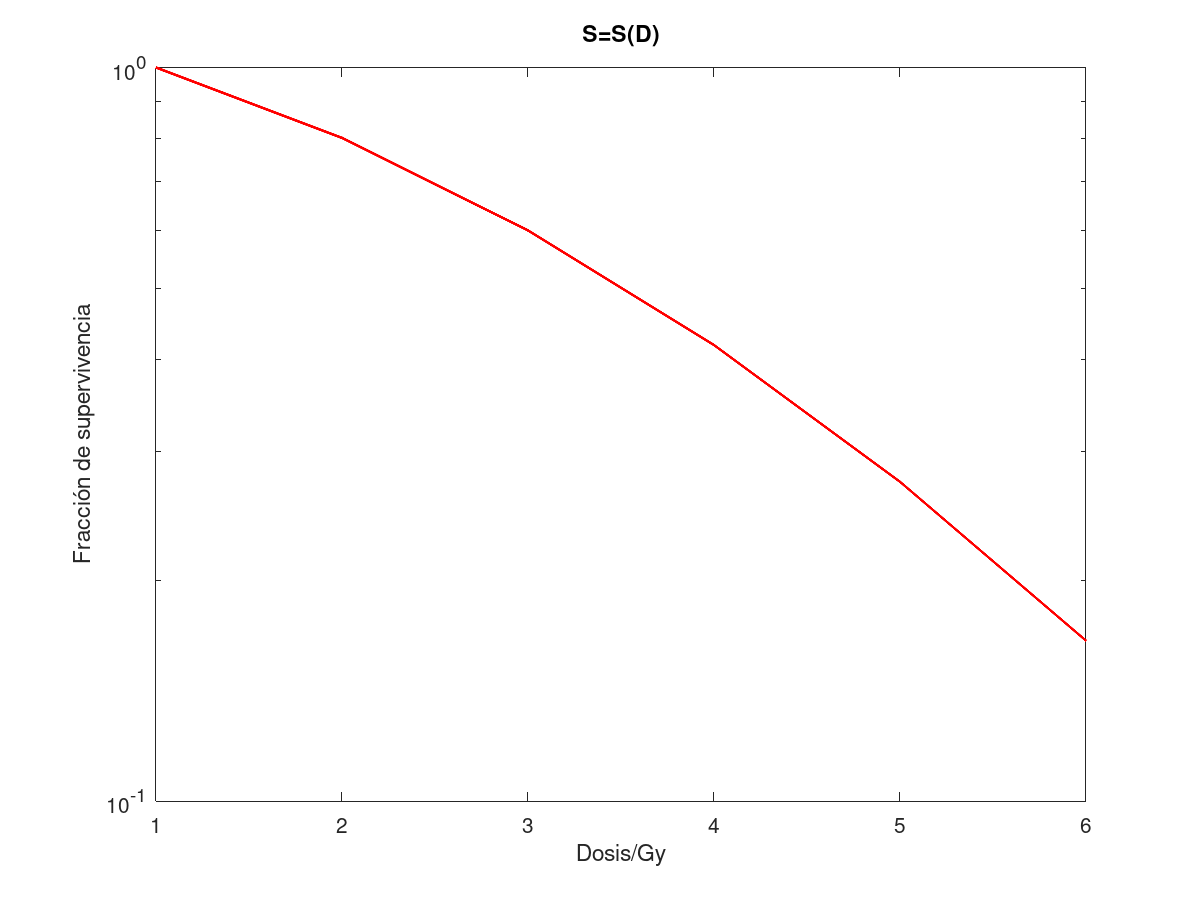
\includegraphics[scale=0.30]{figuras/Csc_toymodel.png}
		\caption{CSC del toy model heurístico generado en \textit{GNU/Octave} con $A=\unit[18.6]{Gy^{-1}}$ y $B=\unit[347]{Gy^{-2}}$ con el eje de dosis en la escala de $10^2$ unidades.}\label{figura_curva_mia}
	\end{figure}  
	
	\chapter{Conclusiones}
	
	El cálculo teórico de los coeficientes de supervivencia celular amerita un estudio profundo de las interacciones de la radiación ionizante con la materia orgánica, pues los efectos biológicos resultantes de dichas interacciones juegan un rol determinante en la evolución de los cultivos y las colonias \textit{in vivo} bajo estudio. Las cinco R de la radioterapia precisan de una definición cuantitativa en términos de la medida en que las células se ven afectadas por el desdoblamiento de las cadenas de ADN en el núcleo celular. Dado que estos procesos son estocásticos, como bien mencionan \cite{Mayles.2007}, \cite{McMahon.2018}, \cite{Hall.2000} entre otros radio-biólogos y biofísicos, la probabilidad de que ocurra un evento letal a través de una colisión directa con los fotones de un haz debe formar parte de esta construcción matemática. 
	
	Los procesos de absorción de energía son una cuestión fundamental termodinámica. Se mantiene interesante la cuestión de cómo modelar las interacciones de la radiación electromagnética (desde una perspectiva corpuscular) en el seno del estudio del calor y sus mecanismos de transferencia así como sus implicaciones a nivel atómico, molecular y, ¿por qué no? sub-atómico. Consideraciones de esta índole podrían, quizá, necesitar una fundamentación termo-estadística o mecánico-cuántica. Y se presenta, naturalmente, como una motivación para seguir estudiando estos procesos. 
	
	El acercamiento heurístico, aunque bien es intuitivo, no revela demasiada información útil sobre los mecanismos de destrucción celular. Pues al no incluir una definición precisa de los efectos biológicos no logra asimilar la naturaleza del fenómeno en cuestión. No obstante, como se puede observar en la figura \ref{figura_curva_mia}, la curva generada por este modelo sigue una forma típica de una CSC como aquellas presentadas en la literatura consultada como \cite{Bleehen.2007}, \cite{Hall.2000}, \cite{Mayles.2007} y  \cite{Tubiana.1990}. Lo que, personalmente, es producto de motivación y un esbozo de haber encaminado bien este proyecto a pesar de la informalidad del modelado. 	

	\bibliography{seminar_bibliography.bib}
	\bibliographystyle{apalike}
	
\end{document}